\documentclass[12pt]{article}

\usepackage{amsmath}
\usepackage[left=1in, right=1in, top=1in, bottom=1in]{geometry}
\usepackage{graphicx}
\graphicspath{ {images/} }

\begin{document}

\title{Takehome Final}
\author{Adam Camilli}
\date{\today}
\maketitle

\begin{enumerate}

\item Consider the network of queues shown in Figure 1 on test. Assume that all arrival and service processes have exponential distributions, and that this system can be modeled as a network of independent M/M/1 queuing systems using Jackson's Theorem. \\
Compute the mean times that a packet spends in each segment of this system, namely $T1 ,T2, T3$ and $T4$,  as well as the average time that a packet spends in the entire system $T$, 
given the arrival rates, service rates and traffic partitioning probabilities given in this figure. (10 points) \\ \\
We are given ($\lambda$s are external):
\begin{align*}
   \lambda_1 &= 10 & \mu_1 &= 20 & p_{Q_1 \rightarrow Q_2} &= 0.4 \\
   \lambda_2 &= 5 & \mu_2 &= 30 & p_{Q_1 \rightarrow Q_3} &= 0.4 \\
   \lambda_3 &= 15 & \mu_3 &= 30 & p_{Q_1 \rightarrow Q_4} &= 0.2 \\
             &\text{}  & \mu_4 &= 25 & p_{Q_2 \rightarrow Q_4} &= 0.3 \\
             &\text{}  & &\text{} &  p_{Q_3 \rightarrow Q_r} &= 0.5 \\
\end{align*}
From this information, we can use Jackson's Theorem to calculate the individual mean arrival times for each queue $Q$:
\begin{align*}
  \lambda_{Q1} &= \lambda_1 &= 10 \\
  \lambda_{Q2} &= \lambda_2 + \lambda_1P_{Q_1 \rightarrow Q_2} &= 9 \\
  \lambda_{Q3} &= \lambda_3 + \lambda_1P_{Q_1 \rightarrow Q_3} &= 19 \\
  \lambda_{Q4} &= \lambda_1P_{Q_1 \rightarrow Q_4} + \lambda_2P_{Q_2 \rightarrow Q_4} + \lambda_3P_{Q_3 \rightarrow Q_4} &= 14.2 \\
\end{align*}
and with them the mean time a packet spends in each segment $T_1$, $T_2$, $T_3$, $T_4$ as well as in the system as a whole:
\[ T_i = \frac{1}{\mu_i - \lambda_i} \]
\begin{align*}
  T_1 &= \frac{1}{20-10} &= 0.1 \\
  T_2 &= \frac{1}{30-9} &= 0.0476 \\
  T_3 &= \frac{1}{30-19} &= 0.091 \\
  T_4 &= \frac{1}{25-14.2} &= 0.0926 \\
\end{align*}
The average time a packet spends in the system as a whole is therefore
\[ T_1 + T_2 + T_3 + T_4 = 0.3312 \text{ sec} \]

\newpage

\item Polynomial codes are typically used for the detection of transmission errors in computer networks. Consider a polynomial code which is based on the CRC-12 generator polynomial $G(X) = X^{12}  +  X^{11}  +  X^3  +  X^2  +  X  +  1$. 
  \begin{enumerate}
  \item Given the message polynomial $M(X) = X^{15} + X^{12} + X^{11} + X^{10} + X^7 + X^5 + X + 1$, compute the corresponding valid code polynomial $T(X)$. \\ \\
    Divisor corresponding to $G(X)$ is 1100000001111. \\ \\
    $r=12$, so append 12 zeroes to message frame corresponding to $M(X)$: 1001110010100011 000000000000
    \begin{align*}
      1100000001111 \text{ }\overline{)1001110010100011000000000000} = & 111100010101011 \\
                                                                       & \text{Rem. }011000001001
    \end{align*}
    Appending remainder to original message now gives us $T(X)$:
    \[ T(X) = 1001110010100011\text{ }011000001001 \]
    
  \item What error patterns can be detected by this generator polynomial, and what fraction of errors can be detected by this generator polynomial? \\ 
    Where $r$ is the degree of G(X) and length of remainder 12:
    \[ \text{Error Fraction } = 1-\frac{1}{2^r} = 1-\frac{1}{2^{12}} \]
  \end{enumerate}

\newpage

\item The distance from the earth to a distant planet is approximately $9 \cdot 10^{10}$ meters.  Assume that a stop-and-wait protocol is used for frame transmission on a 64 Mbps point-to-point link, given that the link is noise-less (error-free), the frame size is 32 Kbytes, the speed of light is $3 \cdot 10^8$ meters/second, and the header size and processing delays at the sender and received are negligible. 
  \begin{enumerate}
  \item What is the channel utilization of the stop-and-wait protocol?  (5 points) \\ \\
    \[ \text{Transmission Time } = \frac{32000 \text{ b}}{64000000 \text{ bps}} = 0.004 \text{ sec} \]
    \[\text{Round Trip Time } = 2 \cdot \frac{\text{Distance}}{\text{Speed}} = 2 \cdot \frac{9\cdot 10^{10}}{3\cdot 10^8} = 600 \text{ sec} \]
    \[\text{Utilization } = \frac{1}{1+2a} = \frac{1}{1+\frac{600}{0.004}} = \frac{1}{150001} \approx 6.667 \cdot 10^{-6} \] 
    
  \item Assume that a sliding window protocol is used instead of the stop-and-wait protocol.  What is the optimum window size for the sender that will achieve maximum utilization of the link?  (4 points) \\ \\
    Optimum window size for sliding window given by 
    \[ W_{opt} = \frac{TT + RTT}{TT} = \frac{0.004+600}{0.004} = 150001 \]
  \end{enumerate}

\newpage 

\item Consider the Go-Back-N and Selective Repeat sliding window protocols given a noise-less (error-free) channel. The frame size is 1000 bytes, headers are short and ACKs are always piggybacked. What is the optimal window size that will achieve maximum channel utilization for these protocols over a 64 kbps satellite channel with a round-trip delay time of 0.54 seconds, and how many sequence bits are required by each protocol to achieve this utilization? (9 points) \\ 
  Given: 
  \begin{center}
    Frame size = 1000 b\\
    Bandwidth = 64000 bps\\
    Round-trip delay = 0.54 sec \\
  \end{center}
  Calculate transmission time from given info:
  \[ \frac{1000 \text { b}}{64000 \text{ bps}} = \frac{1}{64} \text{ sec}\]
  Assuming headers and ACKs are negligible / always piggybacked, our efficiency becomes:
  \[ U = \frac{N}{1+2a}, N = \text{ window size }, a = \frac{0.54}{0.015625} \]
  The window size that will maximize this efficiency is $1 + 2a$ for both protocols. To achieve this:
  \[ \text{Go-Back-N max window size } = 2^n-1 = 1 + 2\frac{0.54}{0.015625} \]
  \[ n = \log_2(71.12) \approx 6 \text{ bits} \] ~\\
  \[ \text{Selective Repeat max window size } = \frac{2^n}{2} = 1 + 2\frac{0.54}{0.015625} \]
  \[ n = \log_2(140.24) \approx 7 \text{ bits} \]

\newpage

\item In the network shown in test, frames are generated at Node A and sent to Node C through Node B.  Nodes B and C acknowledge each data frame immediately upon receipt to Nodes A and B, respectively.  The channel data rate between Nodes A and B is 256 kbps and the data rate between nodes B and C is 1 Mbps. The lines between each pair of nodes are full-duplex, and the propagation delay for each line is 10 $\mu$sec/mile.  All data frames are 1000 bits long and ACKs are separate frames of negligible length.  A sliding window protocol with a window size of W is used between Nodes A and B, and a stop-and-wait protocol is used between Nodes B and C.  All lines are error-free and no frames can be lost. \\ \\
What is the maximum window size $W_{max}$ that can be used between nodes A and B without flooding the buffers of node B?  (9 points) \\ 
Hint:  The buffers of node B will not be flooded if the average number of frames entering and leaving Node B are equal over a long time interval (at steady-state). \\ \\
Given:
\begin{center}
  Propagation Delay = 10 $mu$sec/mi
  Length of frame = 1000 bits
\end{center}
  Considering A to B:
  \begin{center}
    Distance = 2000 mi \\
    Data Rate = 256000 bps
  \end{center}
  Calculate propagation time (A to B):
  \[ 2000 \cdot 10 \cdot 10^{-6} = 0.02 \text{ sec} \]
  and transmission time:
  \[ \frac{L}{R} = \frac{1000}{256000} = \frac{1}{256} sec \]
  Utilization with window size $W$ in a sliding window protocol is:
  \[ U = \frac{W}{1+2a}, a = \frac{0.02}{\frac{1}{256}} \]
  Considering only A to B, the optimal window size would be $1+2a$ to achieve maximum utilization. But now we consider B to C:
  \begin{center}
    Distance = 500 mi \\
    Data Rate = 1000000 bps 
  \end{center}
  Calculate propagation time (B to C):
  \[ 500 \cdot 10 \cdot 10^{-6} = 0.005 \text{ sec}\]
  and transmission time:
  \[ \frac{L}{R} = \frac{1000}{1000000} = 0.001 \text{ sec} \]
  Utilization of a stop-and-wait protocol is:
  \[ U = \frac{1}{1+2a} = \frac{1}{1+2\frac{0.005}{0.001}} = 5 \]
  Since this is the maximum utilization of a stop-and-wait protocol, we must select the window size that corresponds to this so B is not overflooded. Thus our $W_{max}$ is (using $a$ of sliding window protocol):
  \[ 5 = \frac{W_{max}}{1+2a} \Rightarrow W_{max} = 5\left(1+2\cdot\frac{0.02}{\frac{1}{256}}\right) = 56.2 \]
  


\newpage

\item Ten thousand airline reservation stations are competing for the use of a single slotted ALOHA channel. The average station makes 30 requests/hour and a slot is 125 $\mu$sec in duration.  What is the approximate total channel load and resulting throughput? \\
  \[ \text{Average requests of 10000 } = 10000 \cdot \frac{30}{60\cdot 60} = \frac{250}{3} \approx 83.3 \text{ requests/sec} \]
  \[ \text{Channel Load (G) } = \frac{250}{3} \text{ requests/sec }\cdot 0.000125 \text{ sec} = \frac{1}{96} \approx 0.0104 \text{ requests} \]
  Use the formula for slotted ALOHA throughput:
  \[ S_{slotted} = Ge^{-G} = \frac{e^-\frac{1}{96}}{96} \approx 0.0103 \text{ successful requests/sec}\]

\newpage

\item Consider a CSMA/CD LAN with $N$ independent stations. The probability that a station will transmit on an interference interval when given the opportunity is $p$.
  \begin{enumerate}
    \item Derive a formula for the probability $P(A)$ that one and only one station will transmit on an interference interval. (5 points) \\ \\
     Since the $N$ stations are independent, $P(A)$ that only one of the $N$ succeeds is: 
     \begin{align*}
     P(A) = &[P(1 \text{ transmits}) \cdot P(2 \text{ fails}) \cdot P(3 \text{ fails}) \cdot ... \cdot P(N \text {fails})]  +\\
       &[P(1 \text{ fails}) \cdot P(2 \text{ transmits}) \cdot ... \cdot P(N \text{ fails})]  +\\
       & ...         
     \end{align*}
     Given that the probabilities of all of the individual $N$ stations succeding is $p$ and of failing is $1-p$:
     \[ P(A) = Np(1-p)^{N-1} \]

    \item Compute the value of the probability $p$ which maximizes the value of $P(A)$, thereby achieving maximum throughput for this LAN. (4 points) \\ \\
      Using our derived formula, we can examine the results of different $N$:
      \[ N = 2: P(A) = 2p(1-p), \text{ max at } p = \frac{1}{2} \]
      \[ N = 3: P(A) = 3p(1-p)^2, \text{ max at } p = \frac{1}{3} \]
      \[ N = 4: P(A) = 4p(1-p)^3, \text{ max at } p = \frac{1}{4} \]
      This suggests $p = \frac{1}{N}$ to be the value we seek.
    \end{enumerate}

\newpage

\item Consider designing a 2 km-long, 1 Gbps LAN which uses CSMA/CD and has a propagation speed of 200 m/$\mu$sec. What is the minimum frame size and the optimal channel efficiency that can be achieved using this frame size? (9 points) \\ \\
Minimum frame size is equivalent to Bandwidth $\cdot$ Round Trip Time:
\[ RTT = 2 * \frac{2000 \text{ m}}{200 \text{ m/$mu$sec}} = 20 \mu\text{sec} \]
\[ \text{Minimum L } = 20000 bits\]
The optimal channel efficiency is then:
\[ U = \frac{L}{L + RTT} = \frac{20000}{20000 + 20 \mu \text{sec}} = \frac{1000}{1001} \]

\newpage 

\item Assume that the bridges shown in test are transparent bridges, and that all stations have sent and received frames to/from all other stations. Construct the bridge tables for all three bridges. (9 points) \\ \\
Bridge tables tabulate the host addresses they relate, and the network (LAN) number the addreses reside on. Assuming all stations have sent to/from each other:
\begin{center}
  Bridge-1 \\ ~\\
  \begin{tabular}{|c|c|}
    \hline
    Host Address & Network Number \\
    \hline
    A & 1 \\
    \hline
    B & 1 \\
    \hline
    C & 2 \\
    \hline
  \end{tabular} 

  ~\\ ~\\ Bridge-2 \\ ~\\ 
  \begin{tabular}{|c|c|}
    \hline
    Host Address & Network Number \\
    \hline
    A & 1 \\
    \hline
    B & 1 \\
    \hline 
    E & 3 \\
    \hline 
    D & 3 \\
    \hline
    F & 3 \\
    \hline
  \end{tabular} 

  ~\\ ~\\ Bridge-3 \\ ~\\
  \begin{tabular}{|c|c|}
    \hline
    Host Address & Network Number \\
    \hline
    E & 3 \\
    \hline
    F & 3 \\
    \hline
    D & 3 \\
    \hline
    G & 4 \\
    \hline
  \end{tabular} 
\end{center}

\newpage

\item Consider the network shown below.  The numbers shown for each link are the delays between nearest neighbors for that link.  Apply Dijkstra’s algorithm to this network starting at node 1, and label each node with the shortest path route to node 1 using the same label techniques shown in Figure 5-7 in Tanenbaum. (9 points) \\ \\
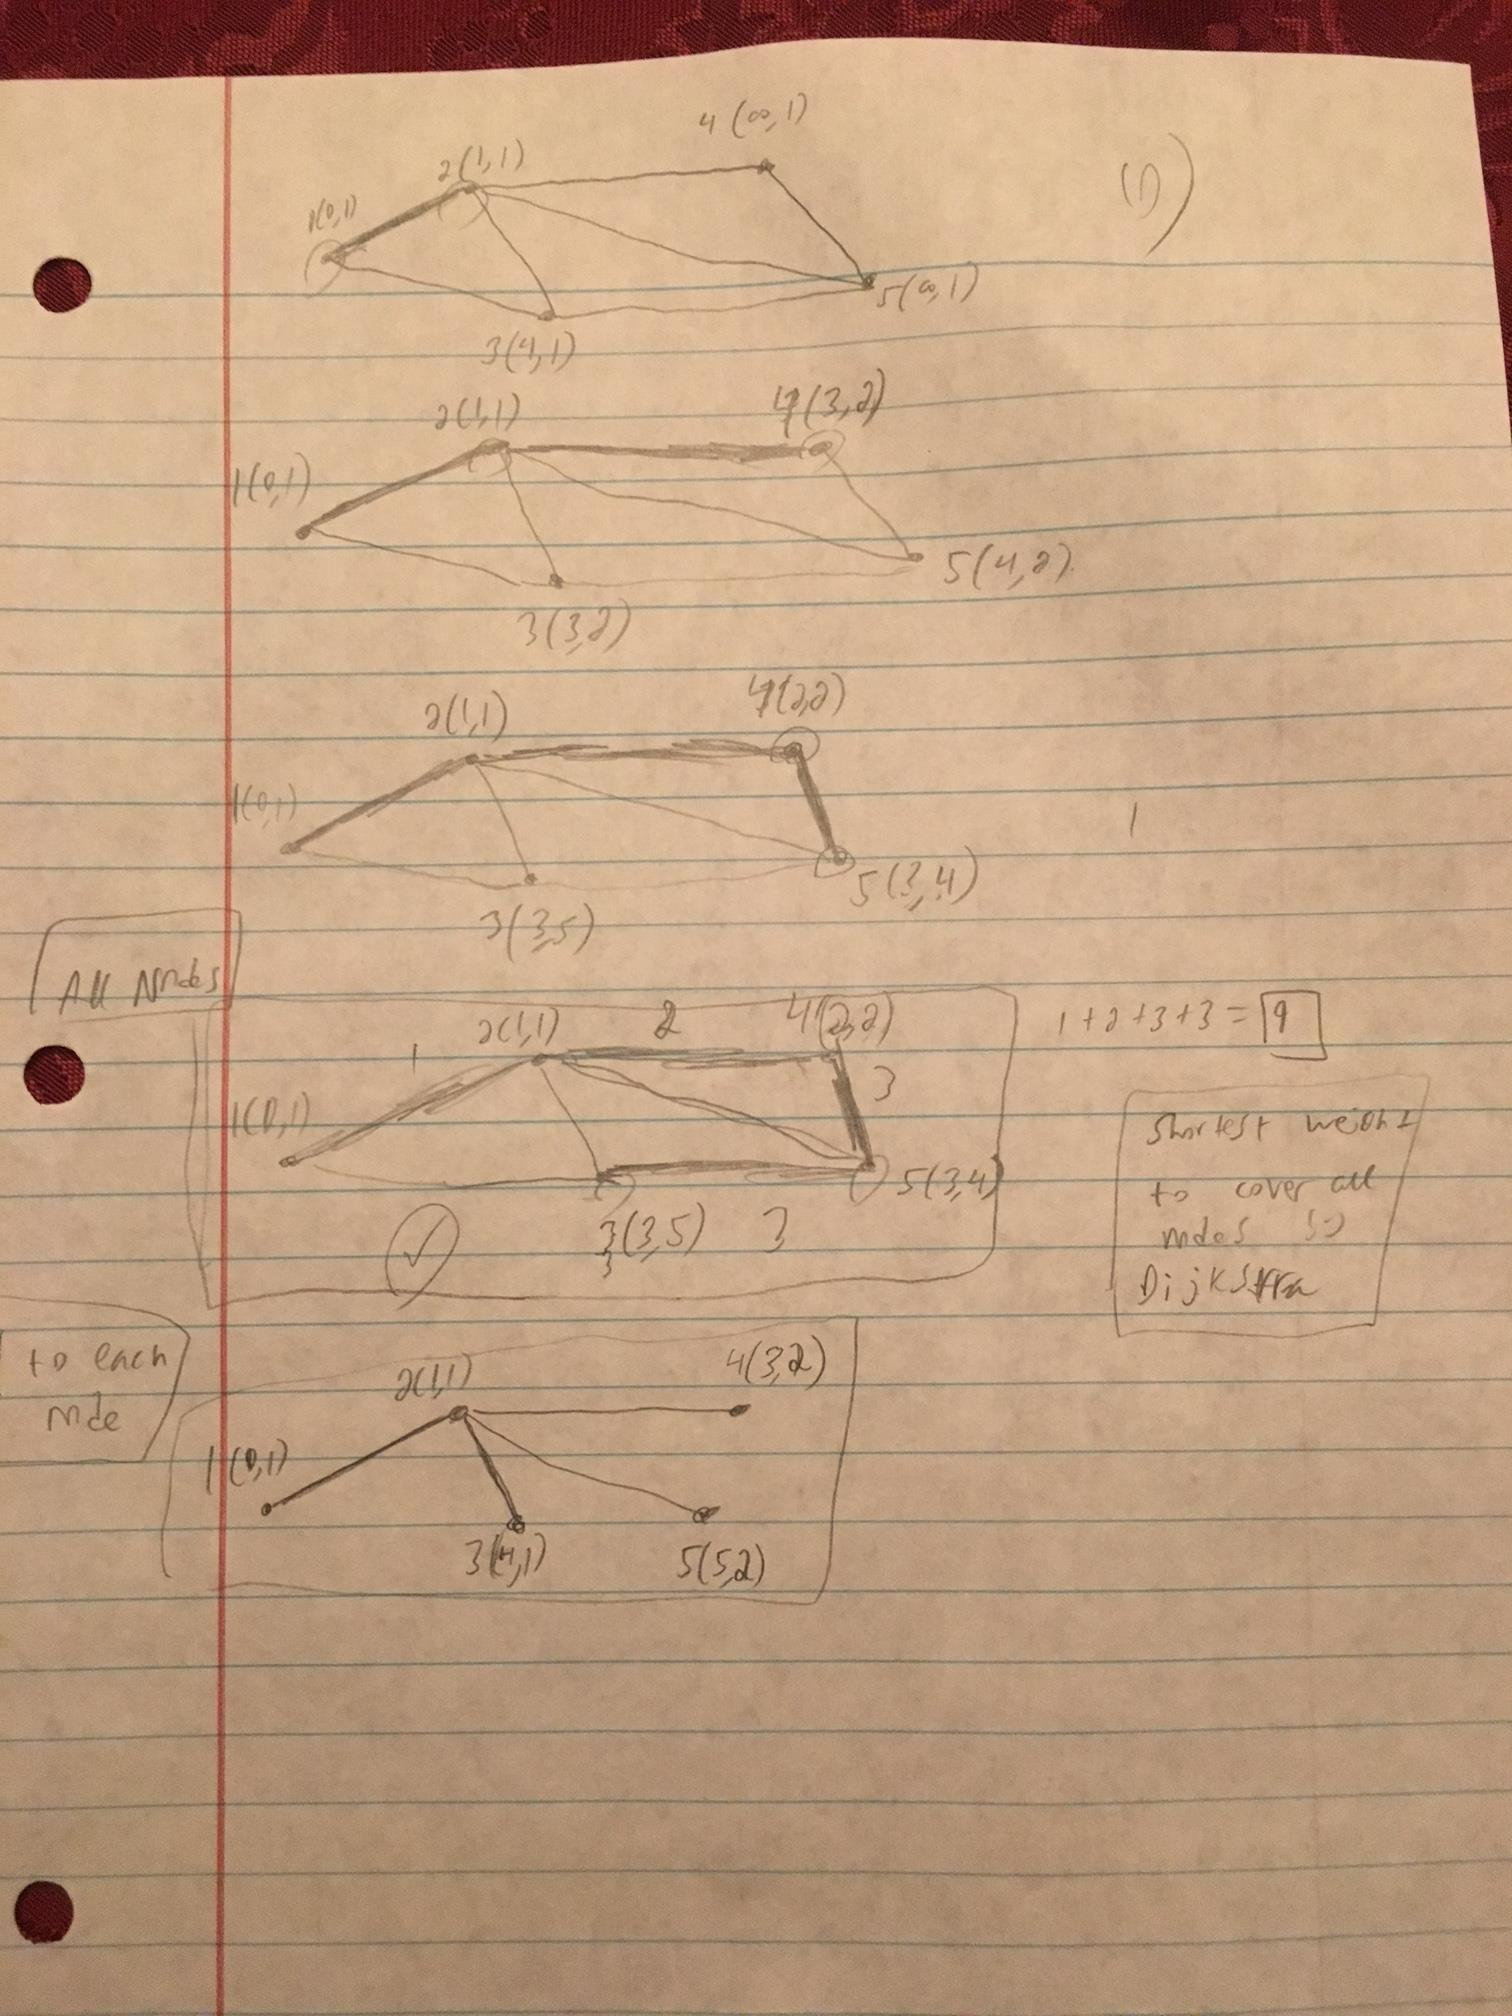
\includegraphics[width=6in, height=8in]{IMG_0194}

\newpage 

\item Assume that that network shown below from Figure 5-7 in Tanenbaum uses link state routing.  The numbers shown for each link are the delays between nearest neighbors for that link.  Construct the link state packets for all eight routers. 
  \begin{center}
    ~\\ ~\\ Link State Packet - A \\ ~\\
    \begin{tabular}{|c|c|}
      \hline
      Neighbor & Delay \\
      \hline
      B & 2 \\
      \hline
      G & 6 \\
      \hline
    \end{tabular} 
    ~\\ ~\\ Link State Packet - B \\ ~\\
    \begin{tabular}{|c|c|}
      \hline
      Neighbor & Delay \\
      \hline
      A & 2 \\
      \hline
      E & 2 \\
      \hline
      C & 7 \\
      \hline
    \end{tabular} 
    ~\\ ~\\ Link State Packet - C \\ ~\\
    \begin{tabular}{|c|c|}
      \hline
      Neighbor & Delay \\
      \hline
      D & 3 \\
      \hline
      F & 3 \\
      \hline
      B & 7 \\
      \hline
    \end{tabular} 
    ~\\ ~\\ Link State Packet - D \\ ~\\
    \begin{tabular}{|c|c|}
      \hline
      Neighbor & Delay \\
      \hline
      C & 3 \\
      \hline
      H & 2 \\
      \hline
    \end{tabular} 
    ~\\ ~\\ Link State Packet - E \\ ~\\
    \begin{tabular}{|c|c|}
      \hline
      Neighbor & Delay \\
      \hline
      G & 1 \\
      \hline
      B & 2 \\
      \hline
      F & 2 \\
      \hline
    \end{tabular} 
    ~\\ ~\\ Link State Packet - F \\ ~\\
    \begin{tabular}{|c|c|}
      \hline
      Neighbor & Delay \\
      \hline
      E & 2 \\
      \hline
      H & 2 \\
      \hline
      C & 3 \\
      \hline
    \end{tabular} 
    ~\\ ~\\ Link State Packet - G \\ ~\\
    \begin{tabular}{|c|c|}
      \hline
      Neighbor & Delay \\
      \hline
      E & 1 \\
      \hline
      H & 4 \\
      \hline
      A & 6 \\
      \hline
    \end{tabular} 
    ~\\ ~\\ Link State Packet - H \\ ~\\
    \begin{tabular}{|c|c|}
      \hline
      Neighbor & Delay \\
      \hline
      D & 2 \\
      \hline
      F & 2 \\
      \hline
      G & 4 \\
      \hline
    \end{tabular} 
  \end{center}
      
\end{enumerate}

\end{document}